\section{Rappels sur la notion de topologie initiale}
On se fixe $E$ un ensemble non vide, $(E_j, \mathcal{T}_j)_{j\in J}$ une famille
d'espaces topologiques et pour chaque $j$ dans $J$ une fonction
$f_j: E\to E_j$.
\begin{df}[Base d'ouverts pour la topologie initiale]\label{init:df}
  On prend comme base d'ouverts les \og rectangles
  ouverts \fg{} suivants:
  \begin{equation*}
    \bigcap_{i\in I}f^{-1}_i(O_i), \mbox{ où }I\subseteq J \mbox{ fini et }
    O_i\in\mathcal{T}_i, \forall i \in I
  \end{equation*}
  Pour rappel, tout ouvert est une union (quelconque) d'éléments
  de la base d'ouverts.
\end{df}

\begin{prop}
  La topologie initiale est la topologie la moins fine
  qui rend les $f_j$ continue.
\end{prop}

\begin{proof}
  On fixe $j\in J$. Soit $O_j$ un ouvert de $\mathcal{T}_j$.
  Alors son image réciproque par $f_j$ est un ouvert
  de la topologie initiale par définition. De plus,
  si une topologie rend continue les $f_j$, elle
  contiendra nécessairement la topologie initiale
  par construction (on vérifie facilement que les
  éléments de la base d'ouverts  de la topologie initiale
  sont ouverts pour la topologie considérée si elle
  rend les $f_j$ continues).
\end{proof}

\begin{prop}\label{init:cont}
  Soient $(F, \mathcal{T}_F)$ et $f: F\to E$ où $E$ est
  muni de la topologie initiale. Alors $f$ est
  continue si et seulement si pour tout $j\in J$,
  $f_j\circ f$ est continue.
\end{prop}

\begin{proof}
  Supposons que $f$ est continue. Alors le résultat est
  immédiat car la continuité est préservée par composition.

  Supposons maintenant que pour tout $j\in J$, $f_j\circ f$
  est continue. Soit $\bigcap_{i\in I}f^{-1}_i(O_i)$,
  où $I\subseteq J$ fini et $O_i\in\mathcal{T}_i$, $\forall i \in I$,
  un ouvert de la base d'ouverts de $E$. Alors
  $$f^{-1}\left(\bigcap_{i\in I}f^{-1}_i(O_i)\right) =
  \bigcap_{i\in I} \left(f_i\circ f\right)^{-1}(O_i)$$
  est, par hypothèse, une intersection finie d'ouverts
  de $F$ (par continuité des $f_i\circ f$, $i\in I$) donc est
  ouverte. Donc $f$ est continue.
\end{proof}
Notez que la preuve fonctionne aussi ponctuellement;
$f$ est continue en $x\in E$ si et seulement si
les $f_j\circ f$ sont continues en $x$ (\textbf{exercice}).
Pour montrer cela
on se rappelle que tout voisinage d'un point contient
un ouvert de la base d'ouverts contenant ce point.

\begin{cor}\label{init:lim}
  Soient $(x_n)_n\subseteq (E, \mathcal{T}_{\mathrm{init}})$ et $x\in E$.
  Alors $x_n\xrightarrow{\mathcal{T}_{\mathrm{init}}} x$ si et seulement
  si pour tout $j\in J$, $f_j(x_n)\xrightarrow{\mathcal{T}_{\mathrm{init}}} f_j(x)$.
\end{cor}

Afin de prouver le corollaire, on montre le résultat suivant (qui
est un rappel):
\begin{lem}\label{lim:topo}
  Soit $(X, \mathcal{T})$ un espace topologique, $(x_n)_n$ une
  suite d'éléments de $X$, et $x\in X$. On munit $\bar{\mathbb{N}}=%
  \mathbb{N}\cup\{+\infty\}$ de la topologie dont une base d'ouverts
  est formée des singletons $\{n\}$ (où $n$ est un nombre naturel)
  et des ensembles de la forme
  $\{n\geq n_0\}\cup\{+\infty\}$, où $n_0\in\mathbb N$.

  Dès lors, $x_n\to x$ si et seulement si l'application
  $n\mapsto x_n$, $+\infty\mapsto x$ est continue en $+\infty$.
\end{lem}

\begin{proof}
  On traduit ce que signifient chacune de ces assertions.
  Dire que cette application est continue en $+\infty$ est,
  par définition:
  \begin{equation*}
    \forall V_x\mbox{ voisinage de $x$},
    \exists V_\infty \mbox{ voisinage de $+\infty$},
    \forall n\in V_\infty, x_n\in V_x
  \end{equation*}
  Dire que $x_n\to x$, revient à dire:
  \begin{equation*}
    \forall V_x \mbox{ voisinage de $x$}, \exists n_0,
    \forall n\geq n_0, x_n\in V_x.
  \end{equation*}
  Il est clair que ces assertions sont équivalentes.
\end{proof}

Le corollaire \ref{init:lim} découle immédiatement de la proposition
\ref{init:cont} et du lemme \ref{lim:topo}.

\subsection*{Exemples}
On rappelle deux exemples vus en deuxième année.
\begin{ex}
  Soit $(X, \mathcal{T})$ un espace topologique et $Y\subseteq X$ un
  sous-ensemble non vide de $X$. Alors, la topologie initiale sur $Y$
  associée à l'injection $Y\hookrightarrow X: y\mapsto y$ est la topologie
  induite.
\end{ex}

\begin{ex}
  Soient $((E_i, \mathcal{T}_i))_{i\in I}$ une famille d'espaces topologiques.
  Soit $E = \prod_{i\in I} E_i$. La topologie initiale sur $E$ associée
  aux projections $p_i: E\to E_i$ est la topologie produit.
\end{ex}


\section{Topologie faible}
Soit $(E, \|.\|)$ un espace vectoriel normé réel. La topologie
faible sur $E$ est une topologie initiale sur $E$.
\begin{df}
  La topologie initiale associée aux éléments de $E^*$
  s'appelle topologie faible sur $E$ et est notée $\sigma(E, E^*)$
  (ou encore $\omega$).
\end{df}

La topologie faible est la topologie la moins fine qui rend les
éléments de $E^*$ continus. En particulier, la topologie faible
sur $E$ vérifie $\sigma(E, E^*)\preceq \mathcal{T}_{\|.\|}$.

\begin{lem}
  Soit $f: E\to\mathbb R$ une application linéaire
  continue au sens de la topologie faible. Alors,
  $f$ est continue au sens de la norme $\|.\|$
\end{lem}

\begin{proof}
  Puisque $\sigma(E, E^*)\preceq \mathcal{T}_{\|.\|}$, et
  que tout ouvert $O$ de $\mathbb R$ vérifie, par
  hypothèse que $f^{-1}(O)\in\sigma(E, E^*)$, le
  résultat est immédiat.
\end{proof}

Les éléments de la base d'ouverts de $\sigma(E, E^*)$ sont de la forme
\begin{equation*}
  \bigcap_{j=1}^n (x_j^*)^{-1}(O_j) =
  \left\{ x\in E\mid \forall 1\leq j\leq n,\quad x_j^*(x)\in O_j\right\}
\end{equation*}
où $n$ est un naturel non nul, $x_j^*$ sont des formes linéaires et continues
sur $E$ et $O_j$ sont des ouverts de $\mathbb R$.

\'{E}tudions les voisinages de $0$. Soit $V_0\subseteq E$ un voisinage
de $0$ au sens de la topologie faible. Alors, il existe $\varepsilon > 0$,
$n\geq 1$ un naturel et $x_j^*\in E^*$, pour $1\leq j\leq n$ tels que
\begin{equation*}
  V_0\supseteq V_{\varepsilon, x_1^*, \ldots, x_n^*}(0) :=
  \left\{ x\in E\mid \forall 1\leq j\leq n,\quad
    |x_j^*(x)| < \varepsilon\right\}
\end{equation*}

\textbf{Explication}: il existe un ouvert $U$ de la base
donnée par la définition de topologie initiale (\ref{init:df})
contenu dans $V_0$, c'est-à-dire
il existe donc un nombre fini (disons $n$) de $x_j^*\in E^*$ et d'ouverts de
$\mathbb R$ contenant $0$ tels que
$U=\bigcap_{j}(x_j^*)^{-1}(O_j)\subseteq V_0$.
Puisque chaque $O_j$ contient un intervalle ouvert centré
en $0$,
on prend pour $\varepsilon$ le minimum des rayons de ces intervalles.
Dès lors, on a:
$$V_{\varepsilon, x_1^*, \ldots, x_n^*}(0)\subseteq U \subseteq V_0.$$

Ceci montre que l'ensemble suivant est un système fondamental
de voisinages de $0$:
$$\left\{V_{\varepsilon, x_1^*, \ldots, x_n^*}(0)\mid \varepsilon > 0,
  n\geq 1, x_j\in E^*, \forall 1\leq j\leq n\right\}. $$

En raisonnant de la même manière, on montre que pour tout $a\in E$,
l'ensemble
$$\left\{V_{\varepsilon, x_1^*, \ldots, x_n^*}(a)\mid \varepsilon > 0,
  n\geq 1, x_j\in E^*, \forall 1\leq j\leq n\right\}$$
est un système fondamental de voisinages de $a\in E$
où $$V_{\varepsilon, x_1^*, \ldots, x_n^*}(a) =
   \left\{ x\in E\mid \forall 1\leq j\leq n,\quad
    |x_j^*(x-a)| < \varepsilon\right\}.$$


\begin{ex}
  Soit $E = \mathbb R^2$. On a vu $E \equiv E^*$.
  Soit $x^*=(x_1, x_2)$ une forme linéaire non nulle sur $E$. L'ensemble
  $\{y = (y_1, y_2)\in \mathbb R^2\mid x^*(y)=0\} = \mathrm{Ker}(x^*)$
  est une droite du plan. Si on fixe $\varepsilon > 0$, on trouve
  que l'ensemble $V_{\varepsilon, x^*}(0)$ est une \og bande\fg dans le plan
  (voir figure \ref{w:ill}).

  En particulier, un tel ouvert contient une droite passant par $0$ et
  tout ouvert de la base d'ouverts est une intersection de telles bandes.
\end{ex}
% Dessin dans le plan d'un ouvert V_epsilon, x^*(0)

\begin{figure}[!h]
  \begin{center}
    \caption{Exemple d'ouvert $V_{\varepsilon, x^*}(0)$ dans le plan}%
    \label{w:ill}
    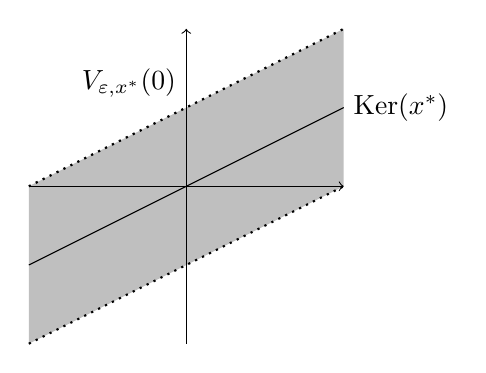
\begin{tikzpicture}
      \draw [->] (0, -2) -- (0, 2);
      \draw [->] (-2, 0) -- (2, 0);
      \draw (-2, -1) -- (2, 1) node[right] {$\mathrm{Ker}(x^*)$};
      \fill [black, nearly transparent] %
            (-2, -2) -- (-2, 0) -- (2, 2) -- (2, 0) -- cycle;
      \draw [dotted, thick] (-2, 0)  -- (0, 1)%
            node[above left] {$V_{\varepsilon, x^*}(0)$}-- (2, 2);
      \draw [dotted, thick] (-2, -2) -- (2, 0);
    \end{tikzpicture}
\end{center}
\end{figure}
On peut généraliser cet exemple: soit $x^*\in E^*$
non nul, alors l'ensemble $V_{\varepsilon, x^*}(0)$ contient un hyperplan
contenant $0$ (car il contient le noyau de $x^*$).

\begin{df}
  Soient $(x_n)$ une suite d'éléments de $E$ et $x\in E$.
  On dit que $(x_n)$ converge faiblement vers $x$ si la suite
  $x_n\xrightarrow{\sigma(E, E^*)}x$ (\emph{i.e.} converge au sens de la topologie
  faible).

  Les notations $x_n\xrightarrow{\omega}x$ et $x_n\rightharpoonup x$ sont
  également employées pour la convergence faible.
\end{df}
\begin{lem}
  Soient $(x_n)$ une suite d'éléments de $E$ et $x\in E$.
  Par le corollaire \ref{init:lim}, pour avoir
  $x_n\xrightarrow{\sigma(E, E^*)}x$,  il suffit de vérifier que pour
  toute forme linéaire $x^*$, on a $$x^*(x_n)\to x^*(x).$$
\end{lem}

Dans le cas d'un espace de Hilbert $H$ sur $\mathbb R$, puisque $H\equiv H^*$
(théorème de Riesz-Fréchet), on a:
$$x_n\xrightarrow{\sigma(E, E^*)}x \iff
\left(\forall y\in H, \langle x_n, y\rangle \to \langle x, y\rangle\right).$$

Il est tout à légitime de se demander s'il y a unicité de la limite
lorsqu'on considère la convergence faible. On a le résultat suivant, qui
assure l'unicité de la limite faible:
\begin{prop}
  $(E, \sigma(E, E^*))$ est séparé.
\end{prop}

\begin{proof}
  Soient $x$, $y$ deux éléments distincts de $E$. Alors $\{x\}$ et
  $\{y\}$ sont deux convexes compacts.
  Par la forme géométrique du théorème de Hahn-Banach, il existe
  un réel $\alpha$, une forme linéaire et continue $x^*$ sur $E$
  tels que $x^*(x) < \alpha < x^*(y)$.
  Alors les ouverts faibles $(x^*)^{-1}(\left]-\infty, a\right[)$
  et $(x^*)^{-1}(\left]a, +\infty\right[)$ contiennent $x$
  et $y$ respectivement et sont clairement disjoints.
\end{proof}

\begin{rem}
  La convergence d'une suite au sens de $\|.\|$ implique la convergence faible
  de cette dernière vers la même limite. Toutefois, l'implication réciproque
  n'est pas vraie en général.

  Soit $\ell^2$ l'espace des suites de carré sommable
  (pour rappel il s'agit d'un espace
  de Hilbert), et la suite $(e_n)_{n\in\mathbb N}\in \ell^2$.

  Cette suite converge faiblement vers $0$, car pour tout élément
  $y$ de $\ell^2$, $\langle e_n, y\rangle = y_n \to 0$ (car
  les termes d'une série convergente convergent vers $0$).
  Toutefois, elle ne converge pas vers $0$ au sens de la norme
  car pour tout $n$, $\|e_n\|_2 = 1$.
\end{rem}

\section{Topologie préfaible}
\subsection{Définition et voisinages}
On se fixe à nouveau un espace vectoriel normé $(E, \|.\|)$. On introduit
une nouvelle topologie sur $E^*$, le dual de $E$, appelée topologie
préfaible. On la notera $\sigma(E^*, E)$ ou encore $\omega^*$.

Il s'agit encore une fois d'une topologie initiale. On considère pour
chaque élément $x\in E$ la fonction linéaire et continue
$$\phi_x: E^*\to\mathbb R: x^*\mapsto x^*(x).$$

\begin{df}
  La topologie initiale sur $E^*$ associée à la famille de fonctions
  $\left(\phi_x\right)_{x\in E}$ est appelée topologie préfaible sur $E^*$.
\end{df}

Les éléments de la base d'ouverts de $\sigma(E^*, E)$ sont
de la forme
\begin{equation*}
  \bigcap_{j=1}^n (\phi_{x_j})^{-1}(O_j) =
  \left\{ x^*\in E^*\mid \forall 1\leq j\leq n,\quad x^*(x_j)\in O_j\right\}
\end{equation*}
où les $x_j$ sont des éléments de $E$ et les $O_j$ des ouverts de $\mathbb R$.

On définit (comme dans la section précédente) pour $a^*\in E^*$ le voisinage
$V_{\epsilon, x_1, \ldots, x_n}(a^*)$ pour $\epsilon > 0$ et
$x_1, \ldots x_n\in E$ comme l'ensemble:
$$ V_{\epsilon, x_1, \ldots, x_n}(a^*) = \left\{
 x^*\in E^* \mid |(x^*-a^*)(x_j) | <\epsilon, \forall j = 1, \ldots, n\right\}.$$
On montre comme pour la topologie faible que l'ensemble de ces voisinages
$$\left\{V_{\epsilon, x_1, \ldots, x_n}(a^*)\mid
  \epsilon > 0, x_1, \ldots, x_n\in E, n\geq 1\right\}$$
est un système fondamental de voisinages de $a^*$.

\subsection{Comparaison de topologies}
On a désormais trois topologies sur le dual de $E$; la topologie forte
(de la norme), la topologie faible $\sigma(E^*, E^{**})$ et la topologie
préfaible $\sigma(E^*, E)$. On peut les comparer comme suit:
\begin{prop}
  On a les comparaisons suivantes:
  $$\sigma(E^*, E) \preceq \sigma(E^*, E^{**}) \preceq \mathcal{T}_{\|.\|}$$
\end{prop}
\begin{proof}
  Au vu de la section précédente, il suffit de vérifier que tout ouvert
  préfaible de $E^*$ est un ouvert faible. Toutefois, puisque
  les $\phi_x$ sont des éléments de $E^{**}$, on en déduit facilement
  que tout ouvert de la base d'ouverts de la topologie préfaible
  est un ouvert de la topologie faible, ce qui donne le résultat.
\end{proof}

\begin{rem}
  Si $E$ est réflexif, alors la topologie faible
  et préfaible sur $E^*$ coïncident.
\end{rem}
\section{Résultats sur la topologie faible}

\begin{thm}
  Soit $(E, \|.\|)$ un espace vectoriel normé.
  Si $E$ est de dimension finie, alors les topologies forte et faible
  coïncident.
\end{thm}

\begin{proof}
  On a déjà $\sigma(E, E^*)\preceq \mathcal T_{\|.\|}$. Il reste à montrer
  l'inclusion réciproque.

  Soit $U\in\mathcal T_{\|.\|}$ un ouvert fort. Il suffit de montrer que
  $U$ est un voisinage faible de tout ses points pour avoir le résultat.
  Soit $x_0\in U$.

  Par hypothèse, il existe $r > 0$ tel que $B(x_0, r)\subseteq U$.
  Pour conclure, il suffit de trouver $\epsilon > 0$ et
  $x_1^*, \ldots, x_m^*\in E^*$ ($m$ à déterminer) tels que
  $V_{\epsilon, x_1^*\ldots, x_m^*}(x_0)\subseteq B(x_0, r)$.

  Notons $n$ la dimension de $E$ et soit $B = (e_i)_{1\leq i\leq n}$ une base
  de $E$ dont tous les vecteurs sont de norme $1$.
  Pour $i = 1, \ldots,  n$, on considère
  $$e_i^*: E\to \mathbb K: x=\sum_{j=1}^nx_je_j \mapsto x_i$$
  (les éléments de la base duale de $B$).

  On recherche désormais $\epsilon > 0$ tel que
  $V_{\epsilon, e_1^*, \ldots, e_n^*}\subseteq B(x_0, r)$.
  Soit $x\in V_{\epsilon, e_1^*, \ldots, e_n^*}$. Alors, on a:
  \begin{IEEEeqnarray*}{rCl}
    \|x - x_0\|&=& \left\|
      \sum_{j= 1}^n e_j^*(x)e_j - \sum_{j= 1}^n e_j^*(x_0)e_j\right\| \\
    & = & \left\|\sum_{j=1}^n e^*_j(x - x_0) e_j\right\| \\
    & \leq &  \sum_{j=1}^n \left|e^*_j(x - x_0)\right| \left\|e_j\right\|
    \leq n\epsilon
  \end{IEEEeqnarray*}
  Il suffit donc de choisir $\epsilon < r/n$.
\end{proof}

\begin{prop}
  Soient $(E, \|.\|)$ un espace de Banach, $(x_n)_{n\in\mathbb N}$ une suite
  d'éléments de $E$ et $x\in E$. Supposons que $(x_n)$ converge faiblement
  vers $x$.
  Alors
  \begin{enumerate}
  \item La suite $(x_n)$ est bornée;
  \item $\|x\|\leq\liminf\|x_n\|$.
  \end{enumerate}
\end{prop}
\begin{proof}
  Pour tout $x^*\in E^*$, la suite $(x^*(x_n))_n$ est bornée car convergente.
  Par la propriété \ref{bs:borne} (découlant du théorème de Banach-Steinhaus),
  la suite $(x_n)_n$ est bornée.

  Pour la seconde partie, on considère $x^*\in E^*$, $\|x^*\|\leq 1$
  Alors, pour tout naturel $n$, $|x^*(x_n)|\leq \|x_n\|$, ce qui
  implique $|x^*(x)| = \liminf|x^*(x_n)| \leq \liminf \|x_n\|$ (notez que
  cette limite inférieure est bien un réel car la suite est
  bornée inférieurement).
  La remarque \ref{hb:a:norme} (un corollaire du théorème de Hahn-Banach)
  assure qu'il existe $x^*\in E^*$, $\|x^*\|\leq 1$ telle que
  $|x^*(x)| = \|x\|$, ce qui donne l'inégalité désirée.
\end{proof}

\begin{prop}
  Soit $(E, \|.\|)$ un espace de Banach. On considère $C\subseteq E$
  un sous-ensemble convexe de $E$. Alors
  $C$ est fermé pour $\sigma(E, E^*)$ si et seulement si $C$ est fermé
  pour la topologie de la norme.
\end{prop}
\begin{proof}
  On peut supposer que $C$ est non vide sans perte de généralité, le cas
  $C = \varnothing$ étant trivial.

  Puisque $\sigma(E, E^*)\preceq \mathcal T_{\|.\|}$, si $C$ est fermé
  pour la topologie faible, alors il est fermé pour la topologie de la norme.

  Réciproquement, supposons que $C$ est fermé pour la topologie de la
  norme. Il faut montrer que $\mathrm{adh}_{\sigma(E, E^*)}(C) = C$.
  L'inclusion $\mathrm{adh}_{\sigma(E, E^*)}(C) \supseteq C$ est toujours vraie
  dans un espace topologique.

  Pour montrer que $\mathrm{adh}_{\sigma(E, E^*)}(C)\subseteq C$, on
  montre plutôt que $(E\setminus C) \subseteq (E\setminus
  \mathrm{adh}_{\sigma(E, E^*)}(C))$. Soit $x\in (E\setminus C)$. Puisque
  $x\notin C = \mathrm{adh}_{\|.\|}(C)$, on peut appliquer une forme géométrique
  du théorème de Hahn-Banach; puisque $C$ est un convexe fermé et $\{x\}$
  est un compact convexe et que ces ensembles sont disjoints,
  il existe $x^*\in E^*$ et un réel $\alpha$
  tels que $x^*(x)< \alpha$ et $x^*(C)\subseteq \left]\alpha, +\infty\right[$.
  En posant $U_x = (x^*)^{-1}(\left]-\infty, \alpha\right[)$, on a un ouvert
  faible tel que $U_x\cap C = \varnothing$ ce qui montre
  $x\notin \mathrm{adh}_{\sigma(E, E^*)}(C)$.
\end{proof}

\begin{prop}
  Soit $(E, \|.\|)$ un espace de Banach de dimension infinie.\\
  Soit $S := S(E) = \{x\in E\mid \|x\| = 1\}$. Alors
  $\mathrm{adh}_{\sigma(E, E^*)}(S) = \{x\in \mid \|x\|\leq 1\}$.
\end{prop}
Avant de prouver la proposition, on introduit le résultat intermédiaire
suivant:
\begin{lem}
  Soit $(E, \|.\|)$ un espace vectoriel de dimension infinie. Soient
  $n\geq 1$ un nombre naturel et $x_1^*$, $\ldots$, $x_n^*\in E^*$.

  Il existe $y_0\in E$ tel que pour tout $i\in \{1$, $\ldots$, $n\}$,
  $x_i^*(y_0)=0$.
\end{lem}

\begin{proof}\label{sph:lem}
  Supposons par l'absurde que pour tout $y\in E\setminus \{0\}$,
  il existe $i\in\{1, \ldots, n\}$, $x_i^*(y)\neq 0$. Alors l'application
  $$\phi: E\to\mathbb{R}^n: y\mapsto (x_i^*(y))_{i=1}^n$$
  est une application linéaire et injective. Dès lors $\dim E\leq n$
  contradiction.
\end{proof}

Prouvons désormais le proposition:
\begin{proof}
  Soit $x_0\in E$, $\|x_0\| < 1$. Montrons que
  $x_0\in \mathrm{adh}_{\sigma(E, E^*)}S$.

  Soit $\epsilon >0$, $n\geq 1$, $x_1^*$, \ldots, $x_n^*\in E^*$,
  montrons que $V:=V_{\epsilon, x_1^*, \ldots, x_n^*}(x_0)$ intersecte $S$.
  Soit $y_0\neq 0$ fourni par le lemme \ref{sph:lem}. On définit une
  application $g:\left[0, +\infty\right[: t\mapsto \|x_0 + ty_0\|$.
  Cette application est continue, $g(0)<1$ et $g$ tend vers l'infini
  quand $t$ tend vers l'infini, il existe $t_0$ tel que $g(t_0) = 1$
  c'est-à-dire $z_0:=x_0 + t_0y_0\in S$.

  Montrons que $z_0\in V$. On a $|x_i^*(x_0 - z_0)|= |t_0x^*_i(y_0)| =
  0 < \epsilon$ par choix de $y_0$, et ce pour tout $i\in\{1$, \ldots, $n\}$.
\end{proof}

\begin{rem}
  On remarque dans la preuve que si $E$ est de dimension infinie,
  tout voisinage (du système fondamental) d'un point $x_0$ contient
  une droite passant par $x_0$, car $x_0 + ty_0$ appartient à ce voisinage
  où $y_0$ est obtenu de la même manière que dans la preuve précédente.
\end{rem}

\begin{exo}
  Soit $(E, \|.\|)$ un espace de dimension infinie. Montrer l'égalité
  $$\mathrm{int}_{\sigma(E, E^*)}(\{x\in E\mid \|x\|<1\})=\varnothing.$$
\end{exo}

\begin{prop}
  Soit $(E, \|.\|)$ un espace vectoriel normé. Alors
  $$(E^*, \sigma(E^*, E))^*\equiv E.$$
\end{prop}
\begin{proof}
  On sait déjà que pour tout $x\in E$, l'application
  $x^{**}: E^*\to \mathbb R: y^*\to x^{**}(y^*) = y^*(x)$ est
  élément de $(E^*, \sigma(E^*, E))^*$ (par définition de la
  topologie préfaible, on retrouve simplement l'application
  qui avait été appelée $\phi_x$).

  Il reste à montrer que pour tout élément $x^{**}$ de
  $(E^*, \sigma(E^*, E))^*$, il existe $x\in E$ tel que
  pour tout $x^*\in E^*$, $x^{**}(x^*) = x^*(x)$.

  Soit $\epsilon=\frac{1}{2}$. Par continuité de $x^{**}$,
  $$U = (x^{**})^{-1}\left(\{\lambda\in\mathbb R\mid
    |\lambda|<\epsilon\}\right)$$
  est un voisinage faible de $0$. Il existe un voisinage de $0$ du système
  fondamental de voisinages énoncé précédemment contenu dans $U$, c'est-à-dire
  il existe $\eta > 0$ et $x_1$,
  \ldots, $x_n\in E$ tels que $V_0:=V_{\eta, x_1, \ldots, x_n}(0)\subseteq U$.

  Soit $x^*\in E^*$. On note ($\star$) l'affirmation suivante:
  si pour tous $i$ allant de $1$ à $n$,
  $x^*(x_i) = 0$, alors $x^*\in V_0$ et $x^{**}(x^*) = 0$.
  L'appartenance $x^*\in V_0$ est claire. Par l'absurde,
  on suppose que $x^{**}(x^*)\neq 0$. Alors $\frac{x^*(x_i)}{x^{**}(x^*)}=0$
  pour tous $i\in\{1, \ldots, n\}$ donc $\frac{x^*}{x^{**}(x^*)}\in
  V_0$ mais
  $x^{**}\left( \frac{x^*}{x^{**}(x^*)}\right)=1\geq\epsilon$ ce qui contredit
  l'inclusion $V_0\subseteq U$.

  Soit $F = \langle x_1, \ldots, x_n\rangle$ et $(x_1, \ldots, x_r)$ une base
  de $F$, $r\leq n$ (quitte à réindicer les $x_i$). Soit pour
  chaque $i$ variant de $1$ à $r$, l'application linéaire et continue
  $x^*_i:F\to\mathbb R$  définie par $x^*_i(x_j) =
  \delta_{i}(\{j\})$ (où $\delta_i$ est le delta de Dirac) pour tous $j$
  allant de $1$ à $r$.
  Par le théorème de Hahn-Banach, chacune de ces fonctions s'étend
  en une fonction $\widetilde{x}_i^*: E\to \mathbb R$.
  On pose $$w^* = x^* - \sum_{i=1}^rx^*(x_i)\widetilde{x}_i^*$$
  (même si ce n'est pas explicitement apparent dans la notation,
  $w^*$ dépend du $x^*$ considéré).

  Pour chaque $j\in\{1, \ldots, r\}$, on a $w^*(x_j)=0$, donc par l'affirmation
  ($\star$), $x^{**}(w^*)=0$. Par linéarité de $x^{**}$, on déduit
  \begin{equation*}
    x^{**}(w^*) = x^{**}(x^*)-\sum_{i=1}^rx^*(x_i)x^{**}(\widetilde{x}_i^*)=0.
  \end{equation*}
  On en déduit
  \begin{equation*}
    x^{**}(x^*)=\sum_{i=1}^rx^*(x_i)x^{**}(\widetilde{x}_i^*)
    = x^*\left(\sum_{i=1}^rx^{**}(\widetilde{x}_i^*)x_i\right),
  \end{equation*}
  et on en déduit que le $x$ recherché est
  $\sum_{i=1}^rx^{**}(\widetilde{x}_i^*)x_i$ (il ne dépend pas
  de $x^*$).
\end{proof}

Notez que dans la preuve précédente, la valeur choisie pour $\varepsilon$
n'a pas d'importance dans les calculs, tant qu'elle est strictement positive.
%%% Local Variables:
%%% mode: latex
%%% TeX-master: "../analyse3"
%%% End:
